%\documentclass{aastex}
\documentclass[iop]{emulateapj}
\usepackage[utf8]{inputenc}
\usepackage{apjfonts}
\usepackage{multirow}

\usepackage{graphicx}
\usepackage{epstopdf}

\newcommand{\myshorttitle}{Near-IR Imaging of M31}
\newcommand{\myshortauthors}{Sick et al.}

\usepackage{color}
\usepackage[pdfauthor={\myshortauthors},pdftitle={\myshorttitle},colorlinks=true,citecolor=blue,linkcolor=blue,urlcolor=blue]{hyperref}
\usepackage{url}

\usepackage{amssymb}
\usepackage{amsmath}

\usepackage{natbib}
\bibliographystyle{apj}

\newcommand{\ie}{\textit{i.e.}}
\newcommand{\eg}{\textit{e.g.}}
\newcommand{\vect}[1]{\boldsymbol{#1}} % vectors or images
\newcommand{\sw}[1]{\textit{#1}} % style software titles
\newcommand{\sn}{\ensuremath{S/N}} % signal to noise
\newcommand{\sersic}{S\'{e}rsic}
\newcommand{\iiwione}{\sw{`I`iwi 1.0}}
\newcommand{\awkward}[1]{\textcolor{red}{#1}}
\newcommand{\todo}[1]{\textcolor{green}{#1}}

% To track draft versions in git
\IfFileExists{vc.tex}{\input{vc}}{}

% aastex setup
\shorttitle{\myshorttitle}
\shortauthors{\myshortauthors}

\begin{document}
    \IfFileExists{vc.tex}{\slugcomment{Version \VCRevision\ by \VCAuthor\ on \VCDateTEX , \VCTime .}
}{\slugcomment{Revision unknown.}}
\title{Near-Infrared Imaging of M31}
\author{Jonathan Sick and Stéphane Courteau}
\affil{Queen's University}
\affil{Stirling Hall, Kingston Canada}
\email{jsick@astro.queensu.ca}

\begin{abstract}
Here is an abstract.
\end{abstract}

\section{Introduction}

Here are some opening thoughts.

\section{Observations}
\label{sec:Observations}

\begin{figure}[t]
	\centering
		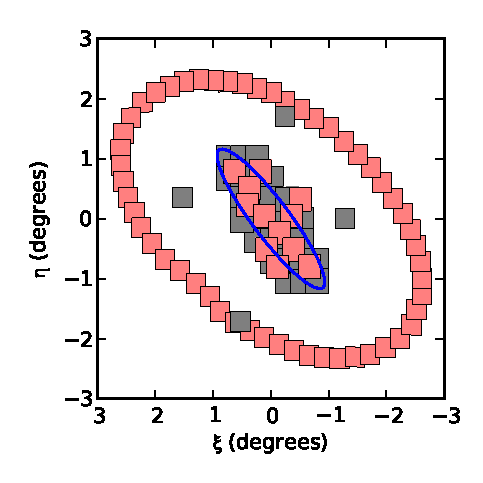
\includegraphics[height=3in]{figs/fieldmap}
	\caption{WIRCam field positions on M31.}
	\label{fig:fieldmap}
\end{figure}

\begin{table*}[t]
    \caption[Summary of WIRCam observing programs]{Summary of WIRCam observing programs. Efficiency (Eff.) is the percentage of time in a program allocated to integrating the disk of M31, compared from nodding, read out and sky overheads. Seeing is measured from stars in sky images.}
    \label{tab:obssummary}
    
    \centering
    \begin{tabular}{llllllllll}
        & & & & $\frac{T_\mathrm{int}}{\mathrm{field}}$ & $T_\mathrm{exp}$ & Eff. & \multicolumn{3}{c}{PSF FWHM (arcsec)} \\ \cline{8-10}
    Sem. & Band & $N_\mathrm{disk}$ & ST Nods & (min) &  (s) &  (\%) & 25th  & 50th & 75th \\
    \hline
    \multirow{2}{*}{2007B} & $J$ & \multirow{2}{*}{27} & [S$^3$T$^8$S$^3$]$^{2}$S$^3$ & 12.5 & 47 & 49 & 0.68 & 0.75 & 0.84 \\
     & $K_s$ &  & [S$^5$T$^{13}$S$^5$]${^2}$S$^5$ & 10.8 & 25 & 42 & 0.60 &  0.65 & 0.73 \\
     \hline
     \multirow{2}{*}{2009B} & $J$ & \multirow{2}{*}{12} & \multirow{2}{*}{[ST$^2$S]$^{20}$S} & \multirow{2}{*}{13.3} & \multirow{2}{*}{20} & \multirow{2}{*}{26} & 0.61 & 0.69 & 0.83 \\
      & $K_s$ & & & & &  & 0.60 & 0.66 & 0.76 \\
    \end{tabular}
\end{table*}

% \begin{deluxetable}{10}
% % \tabletypesize{\small} % or \footnotesize or \scriptsize
% % \rotate
% % \tablewidth{⟨dimen ⟩}
% % \tablenum{⟨text ⟩}
% \tablecolumns{⟨num ⟩}
% \tablecaption{Summary of WIRCam observing programs. Efficiency (Eff.) is the percentage of time in a program allocated to integrating the disk of M31, compared from nodding, read out and sky overheads. Seeing is measured from stars in sky images.
%     \label{⟨key ⟩}}
% \tablehead{⟨text ⟩}
% \end{deluxetable}

The Andromeda Galaxy (M31) was observed in the NIR using the WIRCam instrument, mounted to the 3.6-meter Canada-France-Hawaii Telescope (CFHT), at the summit of Mauna Kea in Hawaii. Observations were carried out exclusively in the NIR $J$ ($\lambda_0 \sim 1.2 \mu\mathrm{m}$) and $K_s$ ($\lambda_0 \sim 2.2 \mu\mathrm{m}$) bands.

WIRCam itself is an array of four HgCdTe HAWAII-RG2 detectors \citep{Puget:2004}. Each detector comprises $2048\times 2048$ pixels, with a scale of 0\farcs 3. This pixel scale critically samples the typical seeing of 0\farcs 65 seen by CFHT. At this pixel scale, M31 stars are well resolved in the halo and outer disk. For reference, $1\arcmin = 3.7\mathrm{pc}$ across the disk of M31. The detectors are arranged in a $2\times 2$ grid with 45\arcsec\ gaps, so that the entire instrument covers $21.5\arcmin \times 21.5\arcmin$ of sky. It is truly the recent advent of NIR focal plane arrays, like WIRCam, that have enabled relatively efficient studies of M31 in the NIR.

In designing our survey of M31, we were driven by two distinct regimes of data reduction and scientific analysis: a high \sn\ image of integrated surface brightness, and resolution of individual Andromeda stars for colour-magnitude diagram analysis. \todo{As discussed in \S}, by simultaneously observing both integrated \emph{and} resolved NIR starlight, we can constrain stellar population synthesis models. Observationally identifying the types of stars that contribute to the NIR light can have profound implications on the inferred masses and ages of distant galaxies.

While the resolved stellar photometry observing regime is straightforwardly accomplished by requesting critical seeing in the Queue Service Observing (QSO) constraints, the integrated surface brightness regime is severely challenged by our understanding of the NIR sky and its spatio-temporal variations (\todo{\S intro}). Originally, we intended for our survey in the 2007B semester at CFHT to accomplish both of these goals. My early analysis, however, suggested that sky background subtraction may not be sufficiently controlled in the those observations, which inspired a second observing campaign in 2009B at CFHT designed to provide tighter constraints on the NIR sky. Thus I describe these two observing campaigns separately in the following sections.

The reader is encouraged to regard these observational designs as \emph{hypotheses} for how to best conduct a wide-field surface brightness survey in the near-infrared from the ground. A goal of this thesis will be to discriminate between the virtues of the 2007B and 2009B programmes, and determine if observational design can improve the construction of a wide-field NIR mosaic.

\todo{ST latency; distance figures}

\subsection{2007B Semester} % (fold)
\label{sec:obs7}

The initial survey was carried out in the 2007B semester by the CFHT Queue Service Observing under photometric conditions. As the observations were designed for resolved stellar analysis, we requested image quality (IQ) of 0.55\arcsec--0.65\arcsec, and our PSF modeling shows this was generally achieved (see Table \ref{tab:obssummary}). This programme covers M31 with 27 contiguous WIRCam fields covering the entirety of M31 out to the optical radius, $\mu_V=23$ mag arcsec$^{-2}$. The fields are arranged with at least 1\arcmin\ overlap in declination, and approximately 5\arcmin\ overlap in right ascension.
% FIXME check overlaps
With the dither pattern (see below), this arrangement yields a continuous mosaic that avoids masked pixels that obscure the eastern 3\arcmin\ of the WIRCam array. The field configuration is shown in Fig. \ref{fig:fieldmap}.

Each field was integrated for $16\times 47 s = 12.5$ minutes in $J$ and $26\times 25 s = 10.8$ minutes in $K_s$. These integrations are sufficiently deep for resolved stellar photometry to reach at least 1 mag below the tip of the red giant branch, a crucial requirement for decomposing the contributions of red giant and asymptotic giant branch stars to the NIR light.

Our surface brightness analysis objective necessitated a regular monitoring of the sky's intensity. Since M31, with a $190\arcmin \times 60\arcmin$ optical disk, is much larger than the WIRCam fields of view, monitoring of the sky zeropoint is only possible by periodically pointing the telescope away from M31, towards blank sky---\emph{sky-target} (ST) nodding. The NIR sky intensity can be expected to change by 5\% in 10 minutes \citep{Adams:1996,Vaduvescu:2004}; since the sky itself is 5 dex brighter than the outer disk of M31 in the NIR, a 5\% uncertainty in the background would be fatal. To constrain the sky to within 1\%, we chose to monitor the sky so that at worst, a sky sample would be no more than 5 minutes removed from a M31 target image. Given the exposure times, this implied a sky (S)--target (T) observing sequence of $S^3T^8S^3$ in $J$ and $S^5T^{13}S^5$ in $K_s$.\footnote{Superscripts here denote the number of times an observation is repeated in sequence for a given target disk field.}

% subsection obs7 (end)

\subsection{2009B Semester} % (fold)
\label{sub:obs9}

Although we had not developed yet sky offset optimization technology described in \S \ref{sec:scalar}, it was apparent that the 2007B data alone would not be sufficient for deep surface photometry of M31. Thus in our 2009B CFHT/WIRCam observing campaign, we set out to perform the \emph{most} exhaustive calibration of M31's NIR surface brightness that could be imagined with a CFHT/WIRCam-class instrument. Our programme was built upon the following axioms:

\begin{enumerate}
    \item \emph{Uncertainty from the temporal variability of the sky must be minimized.} No observation would be delayed by more than 1.5 minutes from a sky sample.
    \item \emph{Systematic uncertainty from the spatial structure of the NIR sky must be minimized.} By visiting many sky fields arranged about M31, we could average over the spatial structure in the sky.
    \item \emph{Uncertainties can be diminished by repeated trials.} Combining more images---each an independent estimate of the disk surface intensity---should reduce the statistical uncertainty of the mean surface intensity, and couplings between fields can be exploited to reduced systematic uncertainties.
    % \item \emph{Systematic sky offsets can be discovered by overlapping both disk and sky fields.}
\end{enumerate}

This reasoning lead to a 2009B observing campaign that included 12 fields on the disk of M31 with 40 repeated observations, integrating for 20 seconds in both the $J$ and $K_s$ bands (13.3 minutes/field/band integration, see Table \ref{tab:obssummary}). Temporal sky variations were minimized with an \emph{inefficient but necessary} ST$^2$S pattern (compared to 2007B: S$^3$T$^8$S$^3$ [$J$] and S$^5$T$^{13}$S$^5$ [$K_s$]). That is, each target observation was directly paired with a sky observation taken within 1.5 minutes (Fig. \todo{lag}). As shown in Fig. \ref{fig:fieldmap}, each target field was overlapped with at least one other 2009B target field so that systematic uncertainties in surface intensities could be checked and corrected. Further, each 2007B disk field overlapped with at least one 2009B disk field so that a surface brightness distribution derived from the 2009B data could be directly used to calibrate the 2007B data.

Throughout the ST nodding pattern, the same sky field was never visited twice for the same target. Nods were semi-randomly assigned towards 53 sky fields, arranged in a ring removed at least 1\arcdeg\ from the optical radius of M31 (Fig. \ref{fig:fieldmap}). In order to maintain rapid telescope nods, only northern sky fields serviced the northern disk, and similar for the southern fields; the maximum offset on the sky was 3\arcdeg\ (see Fig. \todo{todo}). This random sampling of sky fields yielded two possible advantages: 1) when a median sky image is constructed, many \emph{sky shapes} are combined, possibly yielding an intrinsically flatter image of sky (see \S on median sky subtraction), and 2) if there is a coherent structure in the NIR sky, sampling fields of the sky degrees apart in rapid succession should average out these systematic biases in estimating the sky level \emph{on the disk}. Sections \todo{todo} discuss the veracity of these programme design hypotheses.

In their own right, the 2009B sky fields have considerable utility. Over the course of the the 2009B semester, each sky ring field was visited at least five times. Each visit adopted a position from the WIRCam DP5, five-point, dither pattern.\footnote{Implementing a program of random sky nods, while covering a dither pattern on each sky field, proved to be a challenge in the WIRCam phase two proposal interface.} The 100-second integration over each sky field allows deep source masks to be constructed for superior sky flat fielding and median sky subtraction. As an extension to the basic survey, the sky ring fields \texttt{01}, \texttt{13}, \texttt{27} and \texttt{39} were subjected to focussed integration sequences that document the sky variability at a stationary location on the sky over spans of 60--90 minutes. This study is discussed in \S \todo{shapesurvey}. The 50 (45) minute integration in $J$ (and $K_s$) on these fields also allow deep colour magnitude diagrams to be constructed in the inner halo of M31 that complement the optical PAndAS survey \cite{Ibata:2007}.


% subsection obs9 (end)

\section{Image Preparation}
\label{sec:reduction}

Our goal is to produce an accurate mosaic of M31 from ground-based, CFHT/WIRCam, near-infrared images. As is typical, raw images from the telescope are treated by a pipeline that cleans detector signatures and calibrates flux and astrometry. Here we wish to comment on some of image reduction steps that have a significant impact on the quality of our final mosaic.

WIRCam data are offered by CFHT in three progressive stages of \emph{preprocessing} by their \iiwione\ pipeline to allow programmes, such as this one, to re-implement calibration recipes for potentially higher performance. These data flavours are: a raw image that is essentially untouched after leaving the instrument (\texttt{*o.fits}); an image that has been nonlinearity-corrected, dark subtracted and flat fielded (\texttt{*s.fits}); and an image that has been sky subtracted, in addition to all the previous treatments (\texttt{*p.fits}).

As sky subtraction is the highest source of error in this program, the middle data product, \texttt{*s.fits}, would appear most amenable as a starting point for this program. Nonetheless, two \iiwione\ processing stages included in \texttt{*s.fits} products must be handled carefully.

\paragraph{Cross-talk correction.} WIRCam integrations prior to March 2008 (that is, the 2007B data set, but not the 2009B data) suffered from electronic cross talk within the detector. This cross talk is manifested in repeating rings above and below saturated stars.\footnote{See \url{http://cfht.hawaii.edu/Instruments/Imaging/WIRCam/WIRCamCrosstalks.html}.} By default, the \iiwione\ pipeline removes this cross talk by subtracting a median of the 32 amplifier slices. Unfortunately, this algorithm fails in cases where the background has a surface brightness gradient (such as on the disk of M31) and produces an inverse surface brightness gradient that is stronger than the galaxy surface brightness itself. Loic Albert was kind to re-process the 2007B data set with the cross-talk correction turned off.

\paragraph{Flat fielding.} We discovered that the flat fielding offered by \iiwione\ was only accurate to 2\% of edge-to-edge intensity. This appears to be a discrepancy between dome flat fielding, as employed by \iiwione, and night sky flat fielding. A complete discussion of \iiwione\ flat fielding, and the improvement realized by night sky flat fielding, is made in \S \todo{sec:flats}. The introduction of a new field illumination correction necessitates a re-evaluation of the WIRCam photometric zeropoint, as done in \S\todo{sec:photocal}.

\subsection{Night sky flat fielding}
\label{sec:flats}

Images flat-fielded by \iiwione\ show a remarkable amount of fixed structure. In most applications of WIRCam, these detector illumination structures are un-noticed since the median sky subtraction step, to produce the `fully pre-processed' \texttt{*p.fits}, will erase these illumination artifacts from blank sky. That is, median sky subtraction is treated as a secondary flat-field treatment. However, this is a dangerous procedure as illumination corrections must be multiplicative (as it is a correction to the relative efficiency of detecting photons across the WIRCam detector). Employing median sky subtraction only removes observed background signal; it does not correct the efficiency of detecting signal across the detector.

The error introduced by dome flat fielding in the \iiwione\ pipeline may be realized by producing a median stack of sky images (\ie, the same procedure to make sky flats) that have been flat fielded by \iiwione\ preprocessing. While astrophysical sources are eliminated in a median stack, a residual detector structure is revealed that appears to be consistent across WIRCam integrations over time scales of months and years. These structures can be categorized as a detector-scale illumination variation, distinct patches hundreds of pixels across, and horizontal banding that appears to coincide with the 32-pixel high amplifier bands.

We attribute the residual unflatness of \iiwione\ preprocessed products to its use of dome flats. The light path and colour of a reflected tungsten lamp,\footnote{CFHT \iiwione\ manual: \url{http://www.cfht.hawaii.edu/Instruments/Imaging/WIRCam/IiwiVersion1Doc.html}} rather than photons originating from the atmosphere, yields a remarkably different detector illumination calibration. For this project we chose to redo the flat fielding using \emph{sky flats}: flat field images that use the abundant near-infrared sky signal to describe the illumination function of the WIRCam detectors. The procedure for building a sky flat is listed in \S\ref{sec:skyflatpro}.

\subsubsection{Sky flat fielding procedure}
\label{sec:skyflatpro}

\begin{enumerate}
	\item Begin with  \texttt{s.fits} \iiwione\ products (that are dome flat fielded, but not sky subtracted) to take advantage of the \iiwione\ non-linearity correction and dark subtraction. The dome flat fielding is un-done, losslessly, by multiplying the \texttt{s.fits} image with its associated dome flat.\footnote{Dome flats are made available by CFHT, \url{http://limu.cfht.hawaii.edu:80/detrend/wircam/}.}
	\item All un-flattened sky images are procured from our proprietary programme's data set (sky flats could be made more efficiently by CFHT on-site using proprietary images from \emph{all} WIRCam programmes, but this program is itself rich in sky data). The differing levels of field illumination from the sky are standardized by sampling the median intensity in a $400\times 400$ pixel region at the centre of each detector image (with source masking). Each sky detector frame is divided by a factor that brings this central region to $10000$ ADU.
	\item Those standardized sky frames are organized in sets of: filter ($J$ or $K_s$); detector in the array (1--4); and camera run ID (\texttt{QRUNID}) that identifies images taken with continuous WIRCam installation on the telescope. Frames in each group are median combined, pixel-to-pixel. To reduce bias from stars and background galaxies, \sw{Source Extractor} object maps informed weightmaps for each image that effectively mask sources. Median combination of a stack of hundreds of $2048\times2048$ image, each with a weightmap, is computationally expensive. A convenient solution was to use \sw{Swarp} \citep[an image-mosaicing software package,][]{Bertin:2002} in a mode that combined images pixel-to-pixel. These median combined frames were normalized to unit mean intensity.
	\item These sky flats were divided from each sky and disk frame taken under the same conditions (filter, detector and camera installation) to create an illumination-corrected data set.
\end{enumerate}

\noindent Table \ref{tab:flattable} lists the sky flats constructed for this survey.

\begin{table}[t]
    \centering
    \caption{Properties of night sky flats constructed for each Queue Run (\texttt{QRUNID}).}
    \label{tab:flattable}

\begin{tabular}{cccc}
\hline
Filter & QRUNID & $N$ images & $N$ nights \\
\hline
$J$ & 07BQ01 & 24 & 6 \\
$J$ & 07BQ03 & 141 & 9 \\
$J$ & 07BQ05 & 43 & 4 \\
$J$ & 09BQ01 & 111 & 10 \\
$J$ & 09BQ03 & 55 & 3 \\
$J$ & 09BQ08 & 396 & 10 \\
\hline
$K_s$ & 07BQ01 & 35 & 2 \\
$K_s$ & 07BQ03 & 25 & 1 \\
$K_s$ & 07BQ05 & 156 & 6 \\
$K_s$ & 07BQ07 & 133 & 3 \\
$K_s$ & 09BQ01 & 113 & 10 \\
$K_s$ & 09BQ03 & 55 & 3 \\
$K_s$ & 09BQ08 & 637 & 8 \\
\hline
\end{tabular}
\end{table}

\subsection{Sky flat performance}
\label{sec:skyflatstats}

%\begin{figure}[p]
%    \centering
%     \includegraphics[width=\textwidth]{figs/flat/09BQ01_Ks_domeflatratio.pdf}
%    \caption[Dome - sky flat ratio image.]{Percent difference image of the 09BQ01 $K_s$ sky flat to the \texttt{domeflat\_8302B\_20090728HST143302\_Ks} dome flat used in the \iiwione\ pipeline.}
%    \label{fig:domeflatratio}
%    % thesis/flatratio.py
%\end{figure}

\subsubsection{Comparison to \iiwione\ dome flats}


To illustrate the disagreement between the sky and \iiwione\ dome flats, Fig. \todo{fig:domeflatratio} shows a percent difference map of a \iiwione\ dome flat to a sky flat produced via the procedure in \S \todo{sec:skyflatpro}. This map reveals a $\pm2\%$ discrepancy between the two types of flat fields.
% FIXME see thesis/flatratio.py and thesis_plots/ for the flat ratio image.
% In Ks I do see 2\% -- 4\% edge-to-edge.
% TODO repeat this for both $J$ and $K_s$ sky flats.
In practice, the sky flat appears to be the correct description of the WIRCam illumination as application of sky flats \emph{does} remove all types of residual WIRCam illumination features: large scale, small scale, and amplifier band structures.

\subsubsection{Flatness of sky flats}
\label{sec:skyflatshapes}

%\begin{figure}[p]
%	\centering
%		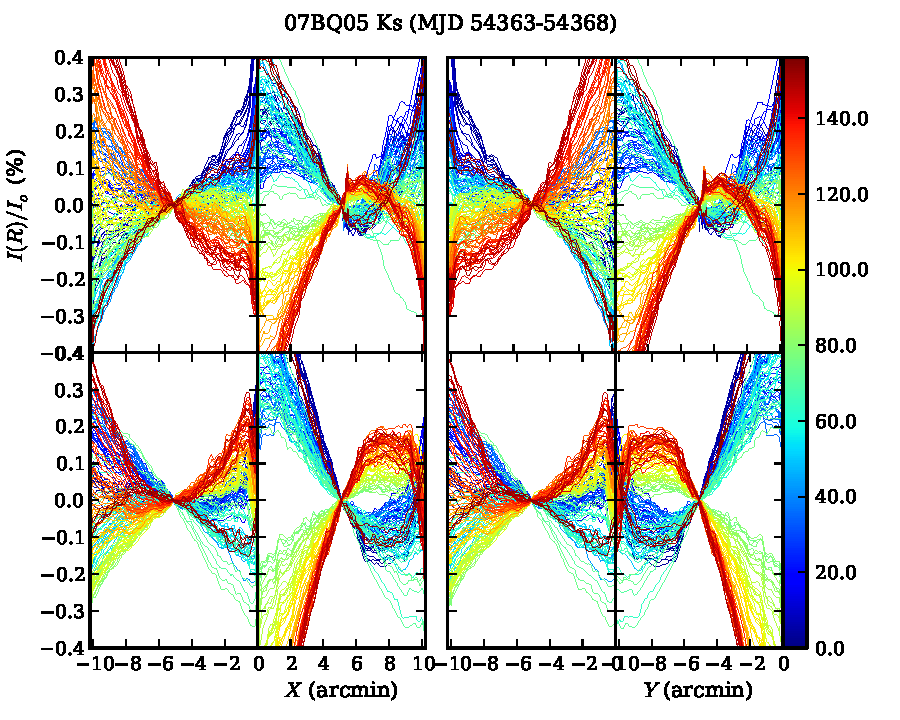
\includegraphics[width=\textwidth]{figs/flat/07BQ05_Ks.pdf}
%	\caption[Sky shape composition of 07BQ05 $K_s$ sky flat]{Evolution of the shapes of sky images composed in the 07BQ05 $K_s$ sky flat. Shape is measured as the median trend across the columns (left array) and rows (right array) WIRCam images. These trends are normalizes to the level at the centre of the detector, $I_o$. Axes are arranged to match the $2\times 2$ configuration of WIRCam. Colours highlight the observation sequence of images.}
%	\label{fig:flat_07BQ05_Ks}
%	% flatshapes.py
%\end{figure}

%\begin{figure}[t]
%	\centering
%		\includegraphics[width=\textwidth]{figs/flat/09BQ08_Ks.pdf}
%	\caption[Sky shape composition of 09BQ08 $K_s$ sky flat]{Sky shape composition of 09BQ08 $K_s$ sky flat. See Fig. \ref{fig:flat_07BQ05_Ks} for explanation.}
%	\label{fig:flat_09BQ08_Ks}
%	% flatshapes.py
%\end{figure}

%\begin{figure}[t]
%    \centering
%        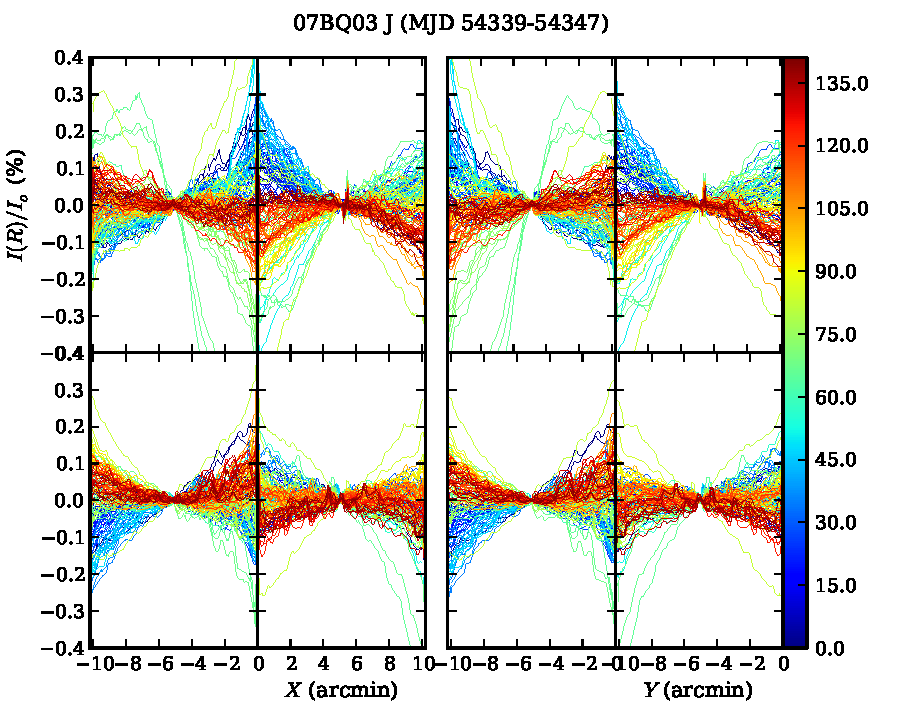
\includegraphics[width=\textwidth]{figs/flat/07BQ03_J.pdf}
%    \caption[Sky shape composition of the 07BQ03 $J$ sky flat]{Sky shape composition of the 07BQ03 $J$ sky flat. See Fig. \ref{fig:flat_07BQ05_Ks} for explanation.}
%    \label{fig:flat_07BQ03_J}
%    % flatshapes.py
%\end{figure}

Ultimately, the accuracy of sky flats is limited by the distribution of intrinsic shapes in the NIR sky. Wide-field movies of the near-infrared sky \citep{Adams:1996} show the NIR sky glow to be akin to a moving cloud system. As such, the NIR sky seen by WIRCam is never flat---yet by definition a flat field must necessarily be built from an intrinsically uniform illumination across the telescope focal plane. In producing a NIR sky flat, we hypothesize that the \emph{mean shape} of the NIR sky, over the span of a queue run, is flat.

In \todo{Figures} \ref{fig:flat_07BQ05_Ks}--\ref{fig:flat_07BQ03_J}, I plot the sequences of sky shapes that are combined to produce a sky flat for typical queue runs of this survey. These `sky shapes' are built by median-compressing the sky images down rows and columns to show the general trend of the sky across $x$ and $y$ image axes. The centre-to-edge shape of the sky, across a 10.4\arcmin\ WIRCam detector, typically varies by 0.1\% in $J$, and 0.5\% in $K_s$. \emph{The performance of dome flats---$\pm2\%$ error relative to sky flats---is worse than the typical uncertainty in shape from a single sky frame.} But the ultimate accuracy of sky flats depends upon the distribution of sky shapes composed in a QSO run. And surprisingly, the shapes are not always randomly distributed, in part because of the sporadic bursts of sky observations throughout a queue run, as the CFHT queued observing program balances several difference observing projects at once.

For example, in 07BQ05 ($K_s$) (Fig. \ref{fig:flat_07BQ05_Ks}), we see distinct traces of sky shapes that correspond to the sporadic activation of this observing program over several nights, for 30 minutes to hours at a time (as is the normal structure of queued observing blocks). Over the span of an \emph{observing block}, the sky will vary slowly. Once the sky is observed again on a different night in a queue run, the sky shape will be vastly different, creating the two distinct sets of shapes. In other cases where more observations are made under different sky conditions, such as 09BQ08 ($K_s$), a more continuous set of sky shapes is observed. In the $J$ band (\eg, Fig. \ref{fig:flat_07BQ03_J}), these distinct sky morphologies are not as pronounced because at the 0.1\% level, the edge-edge sky variation is closer to the intrinsic Poisson pixel noise of the sky (which itself is $\sim 0.1\%$ of the typical $J$ sky intensity per pixel).

%\begin{figure}[p]
%  \centering
%      \includegraphics[height=8in]{figs/flat/flatslices_07.pdf}
%  \caption{Shapes of sky flats across WIRCam detector \#2 for each queue run, in $J$ and $K_s$ compiled in 2007B.}
%  \label{fig:flat_flatslices_07}
%  % flatslice.py
%\end{figure}

%\begin{figure}[p]
%  \centering
%      \includegraphics[height=8in]{figs/flat/flatslices_09.pdf}
%  \caption{Shapes of sky flats across WIRCam detector \#2 for each queue run, in $J$ and $K_s$ compiled in 2009B.}
%  \label{fig:flat_flatslices_09}
%  % flatslice.py
%\end{figure}

One test of the robustness of queue sky flats is to compare the shapes of independent flats from different queue runs. Since WIRCam is removed from the telescope between queue runs, this test effectively provides an upper limit on the bias in the shape built from a finite ensemble of sky images. In figures \ref{fig:flat_flatslices_07} and \ref{fig:flat_flatslices_09} I plot the distribution of vertical and horizontal \emph{slices} through the centre of the sky flats assembled for each QSO run in a given semester, along with the residuals against the median shape. These shapes are from the median of 200 pixel-wide (1\arcmin) slices through the centre of the lower-right detector, and thus resolve specific changes in the perceived detector illumination distribution. I find (queue-) run-to-run shape variations of $\pm$ 0.4\% in both $J$ and $K_s$ bands. Given that the amplitude of $J$ sky variations is only 0.1\% (Fig. \ref{fig:flat_07BQ03_J}), most of the run-to-run flat illumination variation must be intrinsic to changes in the light path. This leaves $<0.1$\% flat field illumination variation attributable to biases in sky shape composition.

\subsection{Median sky image subtraction} % (fold)
\label{sec:mediansky}

Since M31 is much larger than individual WIRCam fields, sky background is subtracted (to first order) using the sky levels found in contemporary sky images. Chapter \ref{ch:obs} describes the sky-target nodding sequences chosen for the 2007B and 2009B observing campaigns. Although a scalar sky level could be estimated from a sky image, and subtracted from the paired target images, it is common to construct a median sky image, the same size as the WIRCam frames, and subtract this 2D image from target images.

This procedure was originally motivated by near-infrared programs where the objects are small, so that the median of several frames in a multi-point dither pattern effortlessly removes the signal flux, leaving only an image of the sky background itself. An advantage of median sky construction is that it not only records the amplitude of a sky signal, but also its \emph{shape}. For large sky-target nods, the recorded shape of the sky will be a less relevant representation of the sky on the target itself. Nonetheless, \iiwione\ retained this practice of median sky construction as a crutch for removing instrumental signals not removed by dome flat fielding (see \S \ref{sec:flats}). With sky flat fielding, this requirement is reduced further. However, median sky subtraction is still useful for building the best images of the sky fields themselves, and it used in the present pipeline. Chapter \ref{ch:planarsky} discusses the influence of median sky subtraction on the shape of residual sky flux on the disk.

Median sky subtraction is implemented as follows:

\begin{enumerate}
	\item For each sky image (termed the primary sky image), five other sky images taken closest in time to the primary image are collected.
	\item From the central $800\times 800$ pixels of each image, the median sky intensity is recorded, $I_{S,i}$. A Source Extractor object mask, as used in \S \ref{sec:flats} for flat fielding, removes bias from astrophysical sources.
	\item Each sky image is additively scaled to a common level of 10,000 ADU, via $\vect{S}_i^\prime =\vect{S}_i + 10000\mathrm{ADU} - I_{S,i}$. This allows differences in overall sky amplitude to be ignored by the median combination.
	\item The median sky frame is constructed from the six scaled sky images using the \sw{Swarp} engine, as described in \S \ref{sec:flats}. Weightmaps built from \iiwione\ pixel masks and Source Extractor object masks are used.
	\item The median sky frame is scaled back to the level of the primary: $\vect{S}_\mathrm{prime} = \vect{S}_\mathrm{median} -10000\mathrm{ADU} + I_{S,\mathrm{prime}}$.
\end{enumerate}

Each image in the data set is sky subtracted by first identifying the median sky frame whose primary image was taken most closely in time. That paired median sky frame is subtracted from the image.

% section mediansky (end)

\subsection{Photometric calibration}
\label{sec:photocal}

The final link in the primary image reduction pipeline is photometric calibration. The intensity $I_\mathrm{ins}$ of each image pixel, measured in analog-to-digital units (ADU), can be converted into an instrumental magnitude, $m_\mathrm{ins}$, via the standard definition $m_\mathrm{ins} = -2.5\log_{10}I_\mathrm{ins}$. Yet instrumental magnitudes cannot be compared from one WIRCam image to another, nor from this data set to others, because of image-to-image changes in detection efficiency. Instead, instrumental protometry is transformed into a standard photometric system via the introduction of a zeropoint,

\begin{equation}
    m_\mathrm{cal} = m_\mathrm{ins} + m_o.
    \label{eq:zpdefinition}
\end{equation}

Given a zeropoint, and with $I_\mathrm{ins}$ counts integrated over $T_\text{exp}$ seconds, the calibrated image is

\begin{equation}
    I_\mathrm{cal} = \frac{I_\mathrm{ins}}{T_\text{exp}} 10^{-2m_o/5},
    \label{eq:fluxcalibration}
\end{equation}

\noindent in units of ADU s$^{-1}$ pixel$^{-2}$, physically interpreted at the relative count rate per pixel if Vega, the reference star, deposits 1 ADU s$^{-1}$ pixel$^{-2}$. Chapters \ref{ch:dcoffset} and \ref{ch:planarsky} use this system to report residual sky subtraction uncertainties.

For this program, it is most convenient establish $m_o$ for each image by bootstrapping to the photometric system of the Two Micron All Sky Survey (2MASS) point source catalog \citep{Skrutskie:2006}. Any WIRCam pointing in the survey contains $\sim 10^2$ stars measured by 2MASS. Although these are not standard stars, the ensemble of 2MASS stars may be treated as such. Given the ensemble difference between instrumental and 2MASS catalog magnitudes of stars, a zeropoint is estimated.

Since the disk of M31 is crowded, and 2MASS has poor resolution (seeing $> 1\arcsec$), 2MASS point source measurements are considered unreliable on the disk. Instead, all zeropoint measurements are made using sky images, and those calibrations are applied to paired disk images (analogous to the median sky subtraction procedure).

\paragraph{Profile-fitting photometry.} Instrumental photometry of 2MASS stars is done using the DAOPHOT suite of profile-fitting software \citep{Stetson:1987}. The photometry code is run autonomously from the author's Python-language pipeline that interfaces to the DAOPHOT software. Doing so allows the 7696 sky frames compiled for this survey to be measured efficiently, while still allowing customized runtime logic in the Python drivers.

For each sky image, stellar photometry begins with the construction of a spatially-dependent model of the instantaneous point spread function (PSF) of CFHT/WIRCam. Stars are detected, and their magnitudes roughly estimated through circular apertures with DAOPHOT. Of these stars, the 100 brightest are selected as candidates for PSF construction. That list is initially culled of stars near flagged pixels (containing bad pixels, diffraction spikes of bright stars, or galaxies) and stars within 40 pixels of a 2MASS star brighter than 14th magnitude (which are saturated in the WIRCam integrations). Using DAOPHOT, a PSF model is iteratively fit to the list of model stars; upon each iteration the spatial-dependence of the PSF model across the image frame is increased from independent to quadratic.

In each PSF-fitting iteration, model stars flagged by DAOPHOT for having poor fits---typically galaxies or blended stars---are culled. Faint stars can contaminate the wings of stellar profiles. At each iteration, known stars are subtracted from the frame using the current PSF model with ALLSTAR \citep{Stetson:1994}. In this clean frame, faint stars that would otherwise be hidden in the wings of bright stars can be detected. PSF fitting itself is performed on an image where all stars \emph{but} the model stars are subtracted.

\paragraph{Aperture corrections.} Given a quadratically-varying PSF model for each sky frame, a catalog of stellar PSF-fitted instrumental magnitudes is made with ALLSTAR. In principle, PSF fitting does not extract the complete flux of a star; stellar images often have faint and extended wings. Photometry with a large circular aperture could in principle detect the entirety of a star's light, but would be subject to a significant increase in background noise in the large aperture. A scheme to avoid increased noise while estimating the total light of a star was developed by \cite{Stetson:1990}. In each sky image, the 40 brightest PSF model stars are measured in 12 photometric apertures monotonically increasing in radius from 3 to 28 pixels. Using this aperture photometry for all model stars in images of a given band, over the course of a night, DAOGROW is used to build growth curves that extrapolate the light of a star to a \emph{total} instrumental magnitude. For each frame, the aperture correction is estimated as the median difference between the total magnitude and the PSF-fitted magnitude over the 40 program stars:

\begin{equation}
    \text{apc} = \langle m_{\text{tot},i} - m_{\text{PSF},i}\rangle .
\end{equation}

\noindent Hence for any arbitrary star in that frame measured by ALLSTAR, its total instrumental magnitude can be estimated as $m_\text{PSF} + \text{apc}$. In this survey, the median aperture correction is $\sim-0.06$ mag, so that $\sim5\%$ of the light of a star is in extended wings not recorded by the PSF model.

\paragraph{2MASS zeropoint estimation.} As discussed, the photometric zeropoint is the systematic difference between WIRCam instrumental and 2MASS photometry. Although several hundred 2MASS stars may be present in a WIRCam frame, only the 2MASS stars corresponding to the PSF model stars are used since these are vetted to be stellar and have clean photometry. Typically $\sim 40$ stars are thus used to estimate the zeropoint for a given frame. For the ensemble of PSF model stars $i$ matched to 2MASS sources, the zeropoint is:

\begin{equation}
    m_o = \langle m_{\text{2MASS},i} +2.5\log_{10}I_{\text{ins},i} - 2.5 \log_{10} T_\text{exp} - \text{apc} \rangle_{i=0\ldots n}.
\end{equation}

For a typical frame, the dispersion of zeropoint estimates about the median is 0.10-0.15 magnitudes. With such an uncertainty, image-to-image variations in zeropoint can be confused with variations in sky level. But under the photometric conditions that these data were recorded, strong zeropoint fluctuations are not expected over short periods. Thus I choose to smooth zeropoints by averaging the zeropoints of frames across a Gaussian-weighted sliding window of width $\sigma=15$ minutes. Such time-averaged zeropoints have uncertainties of $\sim 0.05$ magnitudes.

A future revision of this WIRCam pipeline will solve for colour terms in the zeropoint correction to account for differences between the WIRCam and 2MASS filter sets.

\begin{figure*}[t]
	\centering
		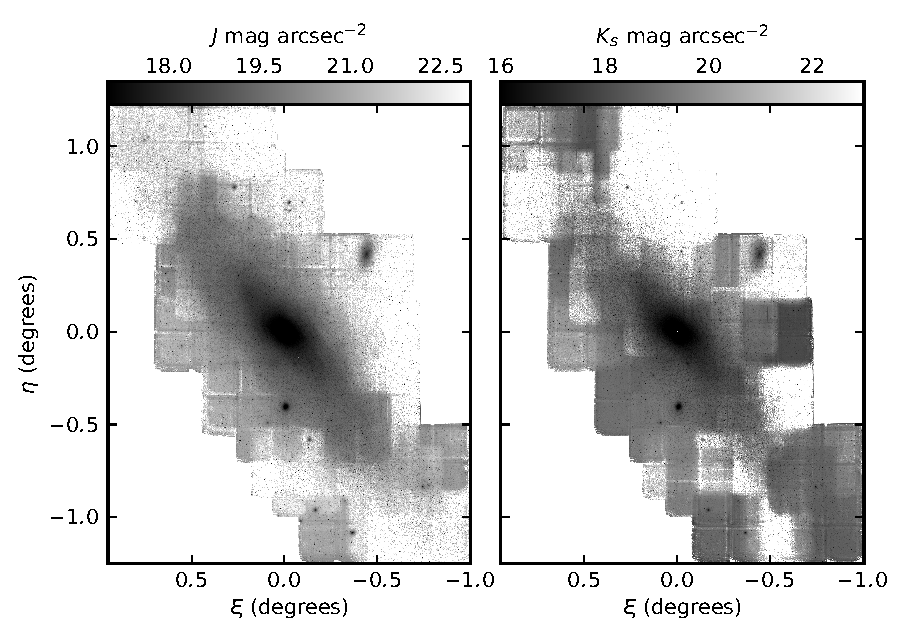
\includegraphics[width=6in]{figs/raw_mosaics}
	\caption{Median sky subtracted WIRCam $J$ (left) and $K_s$ (right) mosaics of M31.}
	\label{fig:raw_mosaics}
\end{figure*}

\section{Scalar Sky Optimization}
\label{sec:scalar}

Despite the best intentions of sky-target nodding (\S obs) and median sky image construction (\S reduction), classical NIR sky subtraction on a target as large as M31 is limited by an uncertainty of 1\% of the sky intensity. Classically, the true value of the sky on the disk of M31 is lost by the temporal and spatial variations of skyglow between disk and sky field observations. Here, we demonstrate that the residual sky bias in each observation can be inferred from information in the overlaps of pairs of images in the mosaic.

Each classically sky subtracted image of the M31 disk is a combination of the true surface intensity, $I_i$, and a residual sky intensity, $\epsilon_i$. Consider a pair of images, $i$ and $j$, that overlap on the galaxy: their difference is $(I_i+\epsilon_i) - (I_j+\epsilon_j) = \epsilon_i - \epsilon_j$. Given this measurement $\epsilon_i - \epsilon_j$ of residual sky intensity, we introduce \emph{sky offsets}, $\Delta$, for each observation so that

\begin{equation}
    (I_i + \epsilon_i - \Delta_i) - (I_j + \epsilon_j - \Delta_i) \rightarrow 0
\end{equation}

\noindent where the intrinsic intensities cancel, $I_i - I_j = 0$. Given a single pair of images, the inference of $\Delta_i$ and $\Delta_j$ is degenerate given the single difference image, $\epsilon_i-\epsilon_j$. But in a mosaic, each image is coupled (has overlapping domain) with many other images, and the mosaic itself can be considered as a network of coupled images. If we model the residual sky intensity $\epsilon_i$ as having a simple shape across the observed images, the single offset $\Delta_i$ will minimize all difference images involving image $i$. That is, sky offsets can be chosen by the non-linear optimization of

\begin{equation}
    \sum_{\forall i,j} [(\epsilon_i - \epsilon_j) - \Delta_i + \Delta_j] \rightarrow 0
    \label{eq:scalartheoryobj}
\end{equation}

\noindent over all coupled pairs $i,j$ in the mosaic.

This algorithm of introducing sky offsets that minimize the differences of all image pairs previously been implemented in the Montage mosaicing package \citep{Berriman:2008}. In that software, 1) images are rectified onto a mosaic pixel grid, 2) difference images are computed, and 3) sky offsets are iteratively chosen by looping through each image pair and choosing the offset needed to minimize the difference image of that pair, counting previous sky offset estimates. Rather than employ Montage for this M31 project, we were motivated to develop a new sky offset optimization algorithms for two reasons: to understand and improve the optimization convergence performance for a large data set, and to deeply understand the systematics and uncertainties of NIR sky subtraction residuals. Given the profound influence of sky residuals on the derived shape of M31's NIR disk, an assessment of uncertainty is crucial. An assessment of errors will be carried out in \todo{\S todo}. The convergence performance of sky optimization algorithms will be addressed in the proceeding sections.

\subsection{Hierarchical sky offset optimization}

Sky offset optimization is challenging because of dimensionality. Assuming that sky residuals are \emph{constant} across a frame (see \S TODO for the case of planar residuals), each image frame represents a new dimension ($\Delta_i$) in the optimization. Considering that the WIRCam array produces four image frames for every exposure, the combined 2007B and 2009B data sets consist of 3924 $J$ and 4972 $K_s$ image frames that cover the disk of M31. Such a large optimization is computationally ambitious, but also needless.

Our sky optimization algorithm breaks the optimization of sky offsets into three sequential steps, which we call \emph{hierarchical sky offset optimization}.

The 2007B and 2009B WIRCam surveys observed a total of 39 \emph{fields} across the M31 disk (illustrated in Fig. \ref{fig:fieldmap}). Each WIRCam field is imaged with four detectors, arranged in a $2\times 2$ grid. Let us define a \emph{detector field} as the collection of images that are taken with a given detector, at a given field. Images in a detector field have the greatly simplifying property of all overlapping across a dominant section of the image frame.

Thus in Step 1 we combine the frames in a detector fild to produce a \emph{detector field stack}. The combined 2007B and 2009B surveys have 156 such stacks per filter. In Step 2, the four detector field stacks within each field can be fitted into a \emph{block}. A block is a fundamental unit of the mosaic, as all images that are combined within a block were observed under contemporaneous sky conditions. Finally, in Step 3, the 39 blocks can be fitted into a galaxy-wide mosaic for each filter.

\todo{Note how the certainty of sky offsets increases with the number of couplings}

\todo{Label the sky offsets that are produced in each step.}

\subsection{Construction of detector field stacks}
\label{sec:stacks}

Scalar sky offsets are most easily computed between the images of a detector field, since individual image frames in a detector field share a common footprint. That is, each image in a detector field is an (approximately) independent random estimate of the true surface brightness of the detector field. The mean surface brightness in the stack of images on a detector field is taken as the best estimate of the actual surface brightness. For each image frame, the difference between the surface brightness of the image and its best-estimate surface brightness of the detector field is taken scalar offset that brings the image to the level of the detector field stack.

The best estimate surface brightness for each detector field stack is first estimated as the mean-combination of all images in a detector field stack.  Since the telescope dithers by a few arcminutes between individual integrations, the edges of the detector field stack have a surface brightness that is estimated from a subset of all the images in a stack. The smaller ensemble of images leads to a visible bias at the stack's edges compared to the middle, where all frames contribute to the surface brightness estimation.

A solution is to estimate offsets for each frame compared to this first detector field stack. Offsets are computed as the median of the difference image between the stack and individual image frames, as described in \todo{Appendix on overlap detection}. The original image frames, now with offsets applied, are re-combined into a detector field stack image. Now edge-effects are smaller. Nonetheless, offsets are estimated a second time to produce a finalized detector field stack image.

\subsection{Non-linear optimization of block and mosaic sky offsets}

The detector field stacking phase (\S \ref{sec:stacks}) created high-\sn\ mosaics of the region covered by a given WIRCam detector at each survey field. Although these detector stacks are best estimates of the galaxy surface intensity at their regions, those stacks have systematic sky surface intensity uncertainties of $\sigma_s$. By combining stacks into blocks (step 2 of the hierarchical offset algorithm) and combining blocks in a mosaic (step 3), those uncertainties are diminished.

Unlike stack production, offseting stacks into blocks and blocks into mosaics requires non-linear optimization since the images do not overlap simultaneously, but rather overlap in a network.

Let us define the objective function that encapsulates the effect of scalar sky offsets on reducing the intensity difference between coupled images:

\begin{equation}
    \mathcal{F} \left(\Delta_1,\ldots,\Delta_n \right) = \sum_{i,j} \mathcal{W}_{ij} \left( \langle \vect{I}_i - \vect{I}_j \rangle - \Delta_i + \Delta_j \right)^2,
    \label{eq:objf}
\end{equation}

\noindent which we intend to minimize by finding the optimal set of scalar sky offsets $\Delta_i$ for each of the detector fields $i$. Note that each coupled image pair is its own term in the objective summation, and that there are as many degrees of freedom ($\Delta_i$) as there are images in the mosaic. Each coupling is tempered by a weighting term $\mathcal{W}_{ij}$:

\begin{equation}
    \mathcal{W}_{ij} = \frac{A_{ij}}{\sigma_{\mathrm{\Delta ij}}},
\end{equation}

\noindent so that more priority is given to couplings of larger areas ($A_{ij}$), and small standard deviations of their difference images ($\sigma_{\Delta ij}$).

Note that the objective function in Eq \ref{eq:objf} puts no constraint on the net sky offset: $\sum \Delta_i$. Assuming that sky subtraction errors are normally distributed, and not biased, sky subtraction offsets should not add a net amount of flux to the mosaic. Fortunately, it is possible to impose this constraint \textit{post facto} by subtracting the mean offset from the sky offsets:

\begin{equation}
    \Delta_i^* = \Delta_i - n^{-1}\sum_{j=1}^n \Delta_j.
    \label{eq:netzero}
\end{equation}

Given the image coupling records, I optimize the set of $\Delta_i$ using the \cite{Nelder:1965} (NM) downhill simplex algorithm. This NM algorithm has the advantage of being naturally multi-dimensional, and being able to work without knowledge of the gradient of the objective function. Instead, the NM algorithm operates by constructing a geometric simplex of $N+1$ dimensions that samples the sky offset parameter space. By evaluating the objective function at each vertex of the simplex, the NM algorithm adapts simplex's shape to ultimately contract upon a minimum.

But NM has two weaknesses. First, it is a \emph{greedy} optimizer that will converge into any local minimum, without necessarily seeking the global minimum. Second, for high-dimension optimizations (many fields in the mosaic), the NM may fail to converge in a reasonable number of objective function evaluations \citep{Neumann:2006}. Without solving these issues, a minimization of Eq \ref{eq:objf} with an off-the-shelf NM code yields a mosaic with obvious discontinuities across fields. To solve the first problem, I develop a Multi-Start Reconverging NM (MSRNM) downhill simplex driver in Appendix \ref{cha:simplex}. This algorithm allows the NM to cumulatively cover a larger portion of parameter space to probabilistically ensure convergence into a global optimum.

\section{Analysis of Scalar Sky Offsets}

\begin{itemize}
\item Maps
\item Hierarchy of offsets
\item Residual flux network maps
\end{itemize}

\begin{figure*}[t]
	\centering
		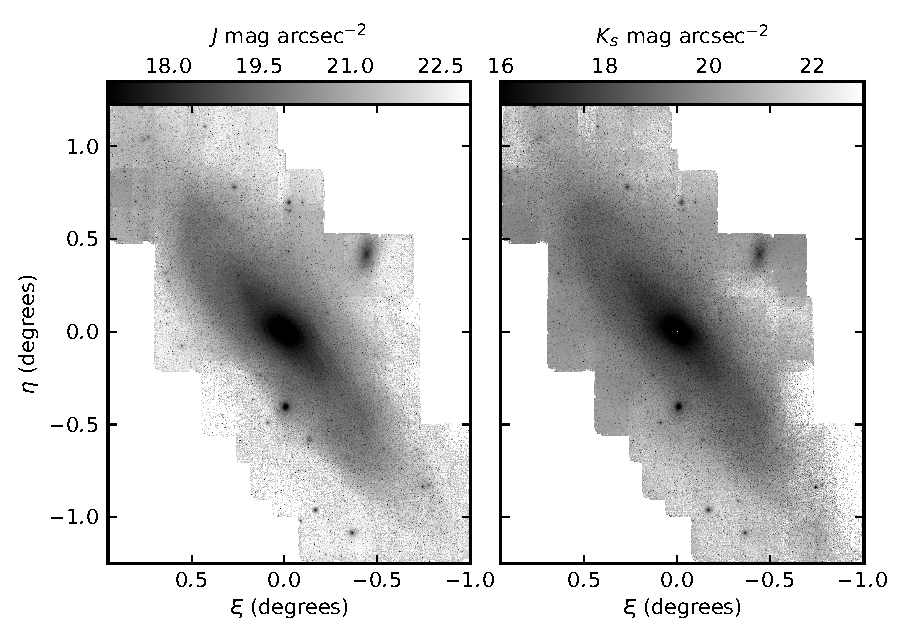
\includegraphics[width=6in]{figs/scalar_mosaics}
	\caption{Scalar-sky fitted WIRCam $J$ (left) and $K_s$ (right) mosaics of M31. Note the qualitative improvement compared to the original, median sky-subtracted, images in Fig. \ref{fig:raw_mosaics}.}
	\label{fig:scalar_mosaics}
\end{figure*}

\section{Planar Sky Offsets}

Scalar sky offsets are greatly effective for recovering the galaxy intensity from sky background uncertainties. But the reconstructed galaxy mosaics (Fig. \todo{maps}) reveal field-to-field discontinuities in the outer disk of roughly the same magnitude as the intrinsic disk surface brightness. These discontinuities are not a failure of the scalar sky offset method to converge; rather, they reveal that residual sky flux has a \emph{shape} across blocks.

Figure \todo{horizontal cut} shows cuts of surface intensity across the $K_s$ scalar-sky corrected mosaic. \todo{Comment on the figure, that blocks have slopes that are not continuous}.

Importantly, these residual sky shape are discontinuous only \emph{between} blocks. Figure \todo{todo} shows surface intensity cuts the component stacks of blocks. None of the blocks show surface intensity breaks between stacks. Recall that stacks within a block are simultaneously observed so that the residual sky present in each stack is correlated. In Table \ref{offset hierarchy table} we realized that $\Delta_\mathrm{stack}$ offsets are minor, and again, we see that sky shape discontinuities within blocks are negligible.

This implies that any endeavor to removed residual sky shapes in the final mosaic need only operate at the block level: scalar sky offsets are an acceptable method for \emph{producing} blocks. In this section would outline such a method where we assume that residual sky shapes can be modeled as planes across blocks. This assumption is consistent with out need to be economical in the dimensionality of optimizations. Since a plane is parameterized as two slopes an a level, the optimization of 39 blocks in each M31 mosaic requires 117 parameters.

\subsection{Planar Sky Offset Optimization Algorithm}

Our planar sky offset optimization algorithm is a direct evolution of the scalar case. As before, difference images are assembled from each coupled pair of blocks. For each difference image we fit a plane $\epsilon_{ij} = (m_x, m_y, c)$: that is, $x$- and $y$-axis slopes and the level $c$ at the center of the difference image. The plane fitting is done iteratively with sigma clipping to reduce the influence of stellar PSF differences of bright stars. Our goal is now to find the sky offset planes for each block, $\Delta_\mathrm{block} = (\Delta_x, \Delta_y, \Delta_c)$, that maximally reduce flux in the difference planes.

The multi-start re-converging Nelder-Mead simplex is again a flexible tool for searching parameter space and finding a global minimum. Planar optimization is more challenging because the parameters in the simplex no longer carry the same meanings, and in particular, have different dynamic ranges. Though we attempted to simultaneously optimize planar slopes and levels by scaling slopes to the same order as levels, that optimization apparatus never converged reliably. Instead, we use an algorithm that iteratively alternates between improving planar levels and slopes until convergence is reached.

Working in the framework of a multi-start optimization, we generate a large suite of random planar offsets that serve as starting points for each optmization `start.' Random planar offsets have levels and slopes drawn from Gaussian distributions $N(0, \sigma_{c,\mathrm{init}})$ and $N(0, \sigma_{x,y,\mathrm{init}})$, respectively. From each initial point, the optimization two Nelder Meade simplex optimizations in succession, each with the ensured reconvergence mechanism (previously described for scalar offset optimiation \S \todo{todo}).

First, planar slopes are optimized. The objective function considers only the minimization of slopes in the difference planes:

\begin{equation}
	\mathcal{F}_m(m_x^0,m_y^0,\ldots m_x^n, m_y^n) = \sum_{i,j} \epsilon_x^{ij} - \Delta_x^i - \Delta_x^j + \epsilon_y^{ij} - \Delta_y^i - \Delta_y^j
\end{equation}

\noindent As done in scalar offset optimization, any converged solution for the best slopes is restarted and reconverged until a stable minimum of the objective functon is found (see \S \todo{restart mechanism}).

Second, the overall levels of offset planes are optimized. This objective function takes the offset slopes derived in the previous step, and seeks to minimize the level, $\epsilon_c$, of difference planes' centers:

\begin{eqnarray}\nonumber
	\mathcal{F}_c(\Delta_\mathrm{block}^0,\ldots,\Delta_\mathrm{block}^n) = &\sum_{i,j}& \mathcal{W}_{ij} [ \epsilon^{ij}_c - (\Delta_c^i + D_x^i\Delta_x^i + D_y^i\Delta_y^i) \\
	&& +~(\Delta_c^j + D_x^j\Delta_x^j + D_y^j\Delta_y^j) ]
\end{eqnarray}

$D_x$ and $D_y$ are distances from the center of the offset plane $\Delta$ to the center of the difference image $\epsilon_ij$. Thus $D_x\Delta_x$ and $D_y\Delta_y$ terms account for the slope's effect on the offset planes level at the center of the $\epsilon_{ij}$ difference image. Again, the restart mechanism is used to ensure a robust minimum of the $\mathcal{F}_c$ objective function.

Together, these two optimization steps produce a new generation of $\Delta_\mathrm{block}$ planar offsets. These new offsets are compared to the previous generation (or the initial random planes for the first iteration) and the fractional difference of each slope and offset is measured. If any fractional difference exceedes a convergence tolerance of 10$^{-7}$, another iteration of optimization is performed. In this iteration, the current planes become new seed planes, and the successive slope and level optimizations are performed. Once an iteration produces planes effectively identical to the previous iteration, the optimization is stopped.

The $N$ optimization starts creates $N$ potential sky offset solutions. To choose the best solution, we seek the solution that minimized the level objective function, $\mathcal{F}_c$. This objective is sensitive to the overall surface intensity difference between coupled fields, while still being dependent on the quality of the planar slopes.

Optimized planar offsets can add a arbitrary amount of flux to a mosaic, and this net offset must be subtracted. Both the net levels and net slopes of the offset planes be subtracted. Given the set of opetimized offset planes, $\Delta$, a \emph{net offset plane} $p$ can be constructed:

\begin{eqnarray}
	p_x & = & n^{-1} \sum_{i=0}^n \Delta_x^i \\
	p_y & = & n^{-1} \sum_{i=0}^n \Delta_y^i \\
	p_c & = & n^{-1} \sum_{i=0}^n \Delta_c^i
\end{eqnarray}

\noindent This net offset plane is subtracted from each optimized offset plane to obtain the final set of planar sky offsets for blocks in the mosaic.

\subsection{Analysis of Planar Sky Offsets}

\bibliography{master}

\end{document}
